\documentclass{article}
\usepackage{graphicx}
\usepackage{pdfpages}
\begin{document}
	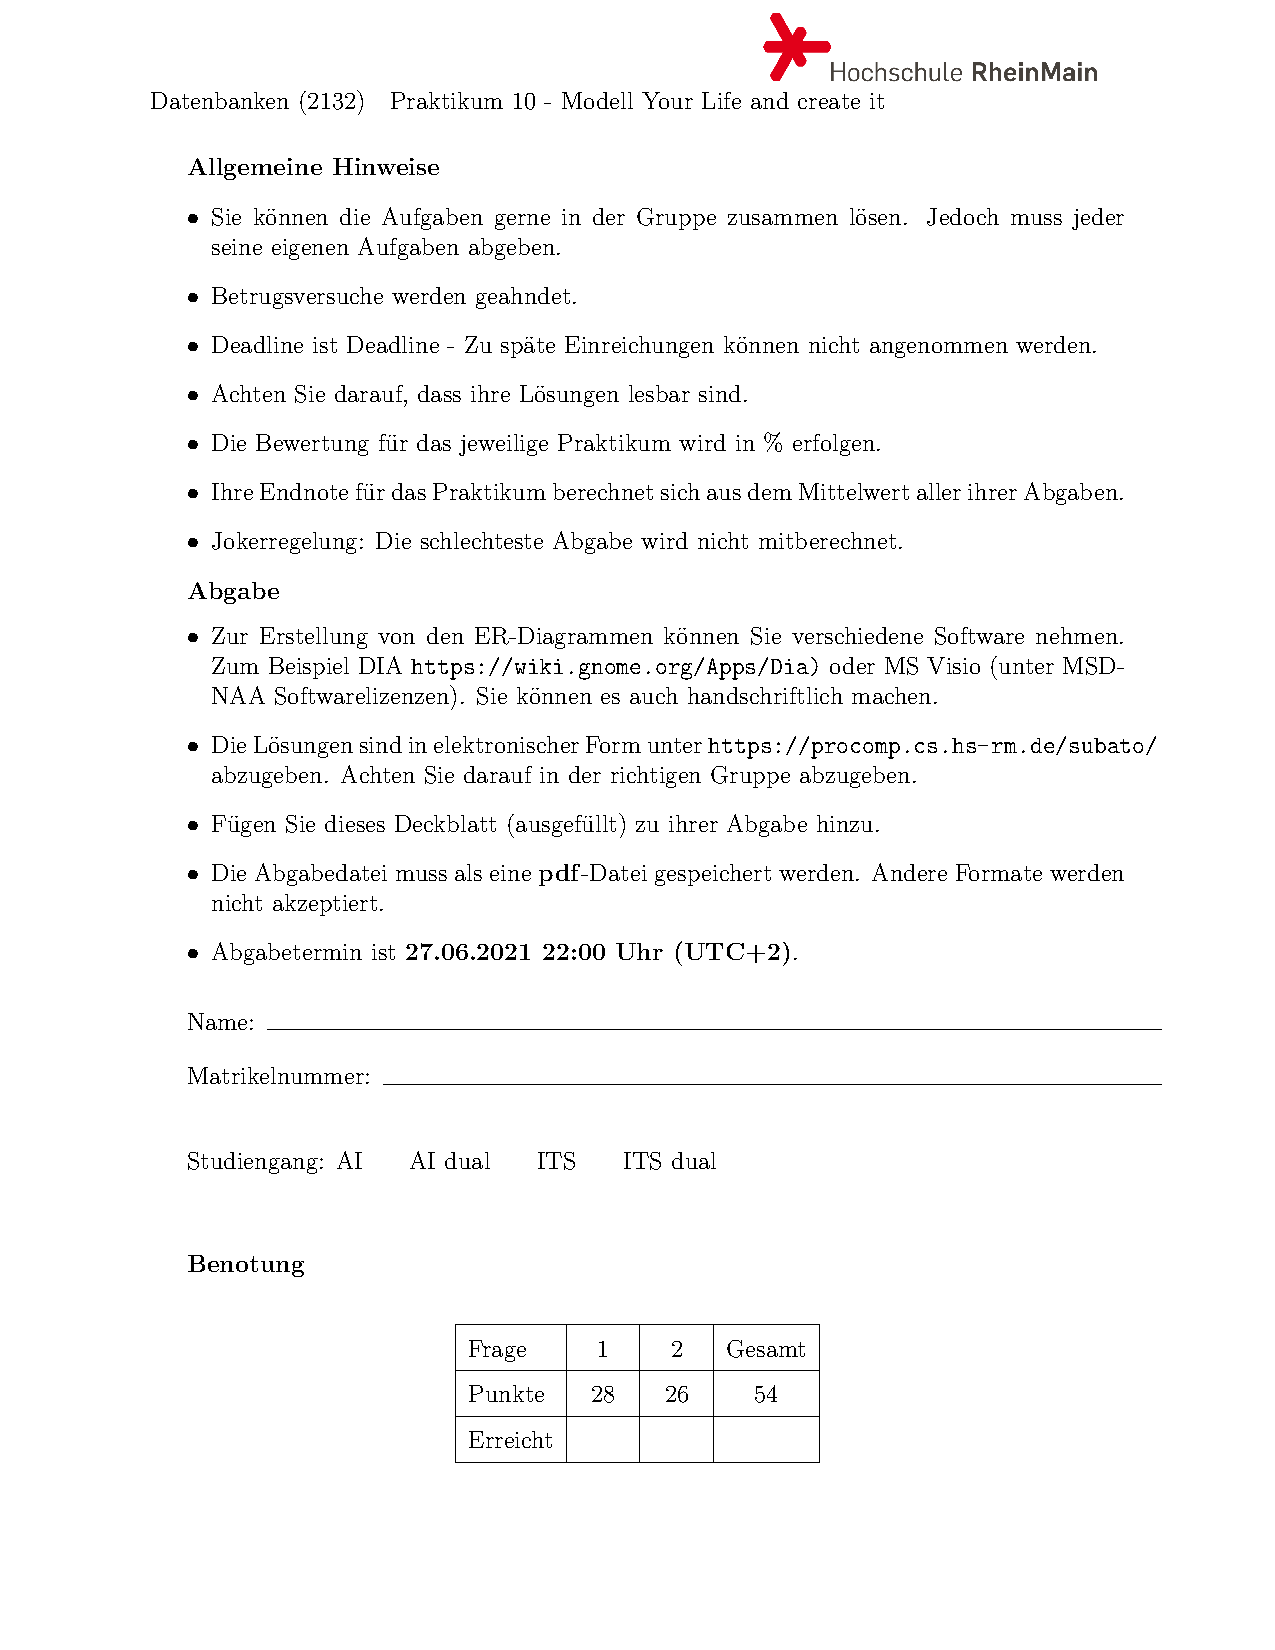
\includepdf[pages=1]{_PA10}
	\section*{Lsg Vorschlag DBÜ10 Maximilian Maag}
	\subsection*{Aufgabe 2}
	\subsection*{a)}
	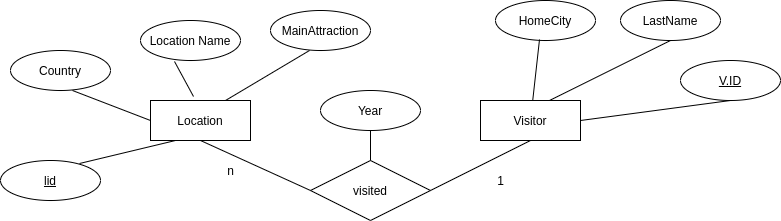
\includegraphics[width=\linewidth]{100201}
	\subsection*{b)}
	Die Datenbank teilt sich in zwei Relationen, die durch die Rhombus Visited verbunden werden. Das zusätzliche Attribut lid in Location und die V.ID sind jeweils eindeutig und bieten sich als Primärschlüssel an. \\
	In der Relationship visited bilden die Fremdschlüssel lid und V.ID einen eindeutigen Primärschlüssel.
\end{document}